\documentclass[a4paper,12pt,oneside]{book}
\usepackage[utf8]{inputenc}
\usepackage{amssymb}
\usepackage{amsmath}
\usepackage{graphicx}
\graphicspath{ {images/} }
\usepackage{times}
\usepackage{geometry}
\usepackage{setspace}
\usepackage{tocloft}
\usepackage{longtable}
\usepackage{array}
\usepackage{booktabs}
\usepackage{tabularx}
\usepackage{fancyhdr}
\usepackage{lastpage}
\usepackage{float}
\usepackage{caption}
\usepackage{subcaption}
\usepackage{listings}
\usepackage{enumitem}
\usepackage{comment}
\usepackage{physics}
\usepackage{algorithm}
\usepackage{algorithmic}

% Page Geometry: 1" top, bottom, right; 1.5" left margin
\geometry{a4paper, tmargin=1in, rmargin=1in, bmargin=1in, lmargin=1.5in}

% Line Spacing: 1.5 throughout
\onehalfspacing

%-----------------------------------------
% Project Metadata & Configuration
%-----------------------------------------
\newcommand{\projecttitle}{Policy-Governed On-Device LLM Agents for Secure Mobile Automation}
\newcommand{\projectid}{PID - 24}
\newcommand{\studentone}{Mekala Karthik}
\newcommand{\studenttwo}{Mohammed Muqeet}
\newcommand{\rollone}{160123729046}
\newcommand{\rolltwo}{160123729047}
\newcommand{\projectdept}{Department of Computer Science \& Engineering (AI \& ML)}
\newcommand{\projectguide}{Dr. Prabhakar Kandukuri}
\newcommand{\guidetitle}{Professor, Department of CSE (AI \& ML)}
\newcommand{\depthod}{Dr. Y. Ramadevi}
\newcommand{\college}{Chaitanya Bharathi Institute of Technology (Autonomous)}
\newcommand{\location}{Gandipet, Hyderabad, Telangana - 500075}
\newcommand{\academicyear}{2026--2027}

% Listings formatting
\lstset{
    basicstyle=\ttfamily\footnotesize,
    breaklines=true,
    frame=single,
    numbers=left,
    numberstyle=\tiny,
    numbersep=8pt,
    captionpos=b,
    tabsize=2,
    showstringspaces=false
}

% TikZ Libraries
\usepackage{tikz}
\usetikzlibrary{arrows, arrows.meta, positioning, shapes.geometric, shapes.misc, calc, shadows}

% Chapter, Section & Subsection Heading Font Specifications:
% 16pt bold for chapter names, 14pt bold for headings (sections), 12pt for normal text
\usepackage{titlesec}
\titleformat{\chapter}[display]
  {\fontsize{16pt}{22pt}\bfseries\centering}
  {\MakeUppercase\chaptertitlename\ \thechapter}
  {8pt}
  {\fontsize{16pt}{22pt}\bfseries\MakeUppercase}
\titlespacing*{\chapter}{0pt}{10pt}{20pt}

\titleformat{\section}
  {\fontsize{14pt}{18pt}\bfseries}
  {\thesection}
  {1em}
  {}
\titlespacing*{\section}{0pt}{12pt}{6pt}

\titleformat{\subsection}
  {\fontsize{13pt}{16pt}\bfseries}
  {\thesubsection}
  {1em}
  {}
\titlespacing*{\subsection}{0pt}{10pt}{4pt}

\titleformat{\subsubsection}
  {\fontsize{12pt}{15pt}\bfseries}
  {\thesubsubsection}
  {1em}
  {}
\titlespacing*{\subsubsection}{0pt}{8pt}{3pt}

% Auxiliary content titles centered
\renewcommand*\contentsname{\Large \centerline{TABLE OF CONTENTS}}
\renewcommand*\listfigurename{\Large \centerline{LIST OF FIGURES}}
\renewcommand*\listtablename{\Large \centerline{LIST OF TABLES}}

% BibLaTeX Setup
\usepackage[
  backend=biber,
  style=numeric,
  sorting=none
]{biblatex}
\addbibresource{reference.bib}

% Page Numbering Specification:
% Bottom center of page in the format: Page 1 of N
\pagestyle{fancy}
\fancyhf{}
\cfoot{Page \thepage\ of \pageref{LastPage}}
\renewcommand{\headrulewidth}{0pt}
\renewcommand{\footrulewidth}{0pt}

\fancypagestyle{plain}{%
  \fancyhf{}%
  \cfoot{Page \thepage\ of \pageref{LastPage}}%
  \renewcommand{\headrulewidth}{0pt}%
  \renewcommand{\footrulewidth}{0pt}%
}

% Indent first paragraph
\usepackage{indentfirst}

% PDF and Hyperref Settings
\usepackage[
  bookmarks=true,
  colorlinks=false,
  pdfborder={0 0 0},
  pdftitle={\projecttitle},
  pdfauthor={\studentone, \studenttwo}
]{hyperref}

\begin{document}

% Frontmatter
\frontmatter
\IfFileExists{titlepage.tex}{\begin{titlepage}
\begin{center}

% Header: A Project Report, VII Semester
\fontsize{14pt}{18pt}\selectfont
\textbf{A Project Report}\\[0.2cm]
\textbf{VII Semester}

\vspace{1.2cm}

% Project Title
\fontsize{20pt}{26pt}\selectfont
\textbf{\projecttitle}

\vspace{1.0cm}

% 'by'
\fontsize{14pt}{18pt}\selectfont
\textbf{\textit{by}}

\vspace{0.6cm}

% Student Names & Roll Numbers
\fontsize{14pt}{19pt}\selectfont
\textbf{\studentone\ (\rollone)}\\[0.25cm]
\textbf{\studenttwo\ (\rolltwo)}

\vspace{1.0cm}

% Guidance Section
\fontsize{14pt}{18pt}\selectfont
\textbf{Under the Guidance of}\\[0.3cm]
\textbf{\projectguide}

\vfill

% Optional College Emblem/Logo (if present in directory)
\IfFileExists{cbit.png}{%
    
\includegraphics[width=1.3in]{cbit.png}\\[0.3cm]
}{\IfFileExists{logo.png}{%
    
\includegraphics[width=1.3in]{logo.png}\\[0.3cm]
}{}}

% Department & College Affiliation
\fontsize{13pt}{17pt}\selectfont
\textbf{Department of CSE( AI \& ML),}\\[0.15cm]
\textbf{Chaitanya Bharathi Institute of Technology (Autonomous),}\\[0.15cm]
\textbf{(Affiliated to Osmania University, Hyderabad)}\\[0.15cm]
\textbf{Hyderabad, TELANGANA (INDIA) -- 500 075}\\[0.35cm]
\textbf{[2026--2027]}

\end{center}
\end{titlepage}
}{}
\IfFileExists{Certificate.tex}{\thispagestyle{empty}

\begin{center}
    
\includegraphics[width=\textwidth]{logo.png}

    \fontsize{16pt}{22pt}\selectfont
    \textbf{CERTIFICATE}
\end{center}

\vspace{0.8cm}

\noindent
\fontsize{12pt}{22pt}\selectfont
This is to certify that the project titled \textbf{``\projecttitle''} is the bonafide work carried out by \textbf{\studentone\ (\rollone)} and \textbf{\studenttwo\ (\rolltwo)}, students of B.E. CSE (AI \& ML) of Chaitanya Bharathi Institute of Technology(A), Hyderabad, affiliated to Osmania University, Hyderabad, Telangana(India) during the academic year 2026-2027, submitted in partial fulfillment of the requirements for the award of the degree in Bachelor of Engineering (Artificial Intelligence \& Machine Learning) and that the project has not formed the basis for the award previously of any other degree, diploma, fellowship or any other similar title.

\vspace{2.5cm}

\noindent
\begin{minipage}[t]{0.5\textwidth}
    \textbf{Supervisor} \\[0.3cm]
    \vspace{0.2cm}
    \projectguide \\
    \guidetitle \\
\end{minipage}
\hfill
\begin{minipage}[t]{0.45\textwidth}
    \raggedleft
    \textbf{Project Coordinator(s)} \\[0.3cm]
    \vspace{0.2cm}
    Dr. K. Mary Sudha Rani \\
    Assistant Professor, Department of CSE (AI \& ML) \\
\end{minipage}

\noindent
\textbf{Place:} Hyderabad \\[0.2cm]
\textbf{Date:}

\clearpage
}{}
\IfFileExists{Declaration.tex}{
\thispagestyle{empty}

\begin{center}
    
\includegraphics[width=\textwidth]{logo.png}

    \vspace{0.3cm}
    \fontsize{16pt}{22pt}\selectfont
    \textbf{Declaration}
\end{center}

\vspace{0.8cm}

\noindent
\fontsize{12pt}{22pt}\selectfont
We hereby declare that the project report entitled
\textbf{``\projecttitle''}, submitted in partial fulfillment of
the requirements for the award of the degree of Bachelor of
Engineering in Artificial Intelligence and Machine Learning,
Chaitanya Bharathi Institute of Technology (A), Hyderabad, is
a record of our own work carried out under the guidance of
\projectguide, \guidetitle. We further declare that all sources
of information used in this report have been duly acknowledged
and cited, and that the report has not been submitted, in part
or in full, for the award of any other degree, diploma,
fellowship or similar title.

\vspace{2.5cm}

\noindent
\begin{minipage}[t]{0.5\textwidth}
    \studentone\ (\rollone)

    \vspace{0.2cm}
\end{minipage}
\hfill
\begin{minipage}[t]{0.45\textwidth}
    \raggedleft
    \studenttwo\ (\rolltwo)

    \vspace{0.2cm}
\end{minipage}

\vspace{0.5cm}

\noindent
\textbf{Place:} Hyderabad \\[0.2cm]
\textbf{Date:}

\clearpage
}{}
\IfFileExists{acknowledgements.tex}{\clearpage
\phantomsection
\addcontentsline{toc}{chapter}{ACKNOWLEDGEMENTS}

\begin{center}
    % 1. Header Image at the very top
    
\includegraphics[width=\textwidth]{logo.png}

    \vspace{0.4in} % Space between logo and title

    % 2. Acknowledgements Title placed below the image
    {\fontsize{16pt}{16pt}\selectfont \textbf{ACKNOWLEDGEMENTS}}
\end{center}

\vspace{0.3in} % Space before your actual text begins

% Your Acknowledgements body text starts here...
\noindent
\fontsize{12pt}{18pt}\selectfont
We express our sincere gratitude to our project guide, \projectguide, \guidetitle, for his valuable guidance, continuous encouragement and constructive feedback throughout the course of this project. His suggestions were instrumental in shaping the direction and quality of this work. \\


\noindent
We thank the Head of the Department, Department of CSE (AI \& ML), and the project coordinators for providing the necessary facilities and an encouraging academic environment. We are also grateful to the faculty and staff of the department for their support, and to our families and friends for their constant motivation during the course of this project. \\



}{}
\IfFileExists{abstract.tex}{\clearpage
\phantomsection
\addcontentsline{toc}{chapter}{ABSTRACT}

\begin{center}
    \IfFileExists{logo.png}{%
        
\includegraphics[width=0.8\textwidth]{logo.png}\\[0.2in]
    }{}

    {\fontsize{16pt}{22pt}\selectfont \textbf{ABSTRACT}}
\end{center}

\vspace{0.3in}

\noindent
\fontsize{12pt}{18pt}\selectfont
Large Language Models (LLMs) have enabled intelligent agents to understand natural-language instructions, reason about tasks, and interact with external tools and system functions. In mobile environments, LLM-based agents can provide convenient automation by allowing users to control device features through natural language. However, providing these agents with access to mobile system capabilities introduces security risks such as unauthorized actions, prompt injection, privilege misuse, and unintended tool execution. These risks highlight the need for secure mechanisms that can control and validate the actions generated by mobile LLM agents.

\vspace{0.2in}
\noindent
This project proposes a Policy-Governed On-Device LLM Agent for Secure Mobile Automation, in which an on-device Small Language Model (sLM) interprets user commands and converts them into structured actions. A policy-governance layer evaluates each generated action based on predefined permissions, risk levels, user intent, and contextual constraints before allowing execution through mobile system APIs. The system is designed to operate fully offline, improving privacy while reducing dependence on cloud services. Its performance will be evaluated using task accuracy, unauthorized-action prevention, attack success rate, response latency,
}{}

% Table of Contents
\clearpage
\phantomsection
\addcontentsline{toc}{chapter}{TABLE OF CONTENTS}
\tableofcontents

% List of Tables
\clearpage
\phantomsection
\addcontentsline{toc}{chapter}{LIST OF TABLES}
\listoftables

% List of Figures
\clearpage
\phantomsection
\addcontentsline{toc}{chapter}{LIST OF FIGURES}
\listoffigures

% Main Content (Chapters)
\mainmatter
%==============================================================================
% CHAPTER 1: INTRODUCTION
%==============================================================================
\chapter{INTRODUCTION}

Mobile smartphones have evolved into the primary personal computing nexus for billions of individuals worldwide, acting as the custodian for confidential communications, biometric identities, financial credentials, health telemetry, and private enterprise data. Concurrently, human-device interaction is undergoing a historic paradigm transition from manual, tactile manipulation of graphical user interfaces toward autonomous, conversational, intent-driven agentic automation. 

Early voice assistants relied upon rigid, handcrafted keyword grammars and intent classifiers that failed to generalize across conversational variations, contextual nuances, and complex multi-step tasks. In recent years, breakthroughs in Large Language Models (LLMs) and post-training quantization techniques have enabled edge-optimized Small Language Models (sLMs) possessing 0.5 billion to 3 billion parameters to execute directly on consumer mobile hardware. When deployed as autonomous agents, these on-device models can parse natural language, reason over device state, and synthesize structured system commands to control operating system features.

However, empowering generative language models with privileged operating system execution capabilities introduces profound security, privacy, and architectural challenges. Non-deterministic token generation is inherently vulnerable to adversarial prompt injection, jailbreaking, instruction deviation, and parameter hallucination. If an autonomous agent directly translates probabilistic model generations into native system tool invocations, the overall security posture of the mobile operating system becomes entirely subordinate to the language model's non-deterministic understanding. This project designs, implements, and evaluates **FLEK** (Fast, Local, Encrypted, Knowledge-governed Agent), a decoupled, policy-governed on-device agent architecture that establishes an unbypassable zero-trust barrier around generative mobile automation.

%------------------------------------------------------------------------------
\section{Problem Definition}
%------------------------------------------------------------------------------

\subsection{Problem Statement and Underlying Challenges}
Traditional mobile operating system security architectures, such as the Android permission framework, are fundamentally static. Permissions (e.g., \texttt{SEND\_SMS}, \texttt{ACCESS\_FINE\_LOCATION}, \texttt{WRITE\_SETTINGS}) are bound declaratively at application installation or requested at runtime. Once granted to an application, the operating system possesses zero semantic insight into whether an individual API invocation is the result of genuine user intent, accidental model hallucination, or adversarial manipulation.

When an autonomous language model agent is granted access to system capabilities, three critical failure modes emerge:
\begin{enumerate}
    \item \textbf{Adversarial Injection and Hijacking:} Language models inherently interleave untrusted input data with control instructions. Adversaries can execute direct prompt injections (e.g., jailbreak framing forcing the agent to exfiltrate contacts) or indirect prompt injections (e.g., hidden instructions embedded in received SMS messages or web pages) that co-opt the agent's decision pathways without the user's knowledge.
    \item \textbf{Syntactic and Semantic Hallucination:} Edge-optimized sLMs operate under strict parameter constraints (1B--3B parameters). Consequently, they exhibit higher rates of hallucinating unregistered tool names, corrupting structured JSON argument payloads, or outputting out-of-bounds parameter values (e.g., setting negative volumes or extreme brightness levels) that can crash native system daemons.
    \item \textbf{Cloud Privacy and Data Egress Dilemma:} Traditional cloud-hosted agent architectures stream private ambient data (such as SMS histories, application state, contact address books, and screen captures) to third-party server farms. This introduces significant roundtrip network latency and violates international privacy regulations, including the General Data Protection Regulation (GDPR) and ISO 27701.
\end{enumerate}

\subsection{Significance of the Project}
The significance of this project lies in bridging the critical gap between conversational AI convenience and rigorous mobile operating system security. By establishing an offline, deterministic policy governance boundary, this work proves that mobile devices can leverage generative agentic intelligence without sacrificing user privacy, system integrity, or battery life. The architecture enforces mathematical and cryptographic execution guarantees that ensure no model hallucination or adversarial prompt can trigger an unauthorized system mutation.

\subsection{Objectives of the Study}
The primary objective of this project is to develop an end-to-end, policy-governed on-device LLM agent architecture for secure Android mobile automation. To achieve this objective, the specific research and engineering goals are:
\begin{enumerate}
    \item \textbf{Air-Gapped Offline Execution:} To deploy a 4-bit quantized Small Language Model (Google Gemma-2B-IT) executing entirely on edge mobile hardware with zero network connectivity and zero cloud data egress.
    \item \textbf{Pre-Inference Semantic Risk Screening:} To design and integrate a lightweight on-device machine learning risk classifier (INT8 MobileBERT) that intercepts adversarial prompts in under 15 milliseconds prior to resource-heavy generative decoding.
    \item \textbf{Syntactic Grammar and Schema Healing:} To construct a context-free GBNF grammar and a deterministic 5-stage syntax healing state machine that guarantees valid structured JSON tool calls from edge sLM outputs.
    \item \textbf{Deterministic Policy Governance (PDP/PEP):} To engineer an independent Policy Decision Point that validates candidate tool invocations against immutable tool whitelists, regex parameter boundaries, dynamic device context (keyguard lock state, night mode caps), and sliding-window rate limits.
    \item \textbf{3-Tier Risk Taxonomy with Human-in-the-Loop (HITL):} To classify mobile actions into three granular risk tiers and enforce mandatory biometric or PIN user confirmation for destructive or privacy-sensitive operations.
    \item \textbf{Single-Use Cryptographic Clearance Protocol:} To formulate a non-bypassable security invariant wherein native Android execution bridges reject any invocation lacking an unconsumed, cryptographically authenticated HMAC-SHA256 clearance token.
    \item \textbf{Tamper-Evident Forensic Audit Ledger:} To implement an on-device SQLite audit store utilizing parent-child SHA-256 hash chaining to provide non-repudiation and immutable execution provenance.
    \item \textbf{Empirical Mobile Benchmarking:} To conduct extensive physical hardware evaluations on Android 14 measuring Task Accuracy, Unauthorized Action Prevention Rate (UAPR), Attack Success Rate (ASR), execution latency, and memory consumption across 105 standardized test scenarios.
\end{enumerate}

%------------------------------------------------------------------------------
\section{Methodologies}
%------------------------------------------------------------------------------

The methodological foundation of FLEK is rooted in the **Zero-Trust Principle** applied to generative language models. The computational architecture is explicitly partitioned into two security domains: an **Untrusted Domain** (comprising raw user queries, external context, and the generative sLM) and a **Trusted Computing Base (TCB)** (comprising the pre-inference risk classifier, deterministic Policy Governance Engine, Hardware Keystore, and native Android tool bridges).

The overall methodology executes through five coordinated pipeline stages:
\begin{enumerate}
    \item \textbf{Stage 1: Pre-Inference Risk Triage:} Raw user text is screened by a lightweight discriminative MobileBERT INT8 classifier. Prompts exhibiting high adversarial risk scores ($\ge \theta_2$) are aborted immediately, neutralizing Denial-of-Service (DoS) compute exhaustion attacks.
    \item \textbf{Stage 2: Air-Gapped Generative Intent Planning:} Cleared prompts are forwarded to an air-gapped on-device sLM (Google Gemma-2B-IT INT4 via Google MediaPipe GenAI). The model operates without the \texttt{android.permission.INTERNET} manifest declaration. Its output is constrained by a GBNF grammar and processed by a syntax-healing state machine to emit a strongly-typed candidate action payload: $A = \langle a_{\text{id}}, P \rangle$.
    \item \textbf{Stage 3: Deterministic Policy Evaluation:} The Policy Decision Point (PDP) evaluates the candidate action against active device context $C$. If the action is registered, satisfies argument boundaries, respects context invariants, and does not exceed rate limits, the PDP approves the request. If the action belongs to Tier 3 (High Risk), the Policy Enforcement Point (PEP) triggers a native Android biometric prompt for explicit Human-in-the-Loop authorization.
    \item \textbf{Stage 4: Cryptographically Verified Native Dispatch:} Upon approval, the policy engine mints a single-use HMAC-SHA256 clearance token $\tau$ using an ephemeral key from the Android Keystore. The Action Dispatcher verifies token authenticity and freshness before invoking native Android platform channels to execute the underlying system APIs.
    \item \textbf{Stage 5: Forensic Audit Persistence:} Every pipeline event—spanning raw query, risk score, sLM plan, policy evaluation metrics, cryptographic token hash, and execution outcome—is appended to an on-device SQLite ledger using parent-child SHA-256 hash chaining ($h_i = \text{SHA-256}(h_{i-1} \,\|\, r_i \,\|\, \tau_i)$).
\end{enumerate}

%------------------------------------------------------------------------------
\section{Outline of the Results}
%------------------------------------------------------------------------------

The FLEK architecture was fully implemented in Flutter (Dart) and native Android (Kotlin) and evaluated on a physical Qualcomm Snapdragon 778G mobile testbed running Android 14. Empirical benchmarking was conducted across a standardized 105-prompt test suite comprising normal commands ($n=32$), ambiguous commands ($n=26$), direct malicious/jailbreak attacks ($n=26$), and parameter boundary fuzzing attacks ($n=21$).

The key experimental findings are:
\begin{itemize}
    \item \textbf{Complete Adversarial Neutralization:} While an ungoverned sLM baseline suffered an alarming **55.3\% Attack Success Rate (ASR)**, the proposed FLEK system achieved a **0.0\% ASR** and a **100.0\% Unauthorized Action Prevention Rate (UAPR)**, intercepting all 47 adversarial and boundary fuzzing vectors.
    \item \textbf{High Task Accuracy:} FLEK achieved an overall task completion accuracy of **96.2\%** on legitimate and ambiguous commands, correctly executing system adjustments and gracefully handling underspecified queries via conversational fallback.
    \item \textbf{Negligible Security Latency Overhead:} Microsecond-level instrumentation revealed that the deterministic Policy Decision Point introduces an average latency of only **0.42 ms**, representing just **0.16\%** of total roundtrip execution latency (262.1 ms). Total security screening (including the 12.4 ms MobileBERT classifier) constitutes under 6\% of total execution time.
    \item \textbf{Minimal Auxiliary Memory Footprint:} The entire security governance infrastructure requires only **32.5 MB** of auxiliary RAM, coexisting smoothly with the 4-bit quantized Gemma-2B-IT model (1.38 GB resident RAM) without triggering Android Low Memory Killer (LMK) interruptions.
\end{itemize}

%------------------------------------------------------------------------------
\section{Scope of the Project}
%------------------------------------------------------------------------------

The scope of this Phase 1 Major Project encompasses:
\begin{enumerate}
    \item Designing, formalizing, and deploying an on-device, zero-egress mobile automation agent on Android (API level 28+).
    \item Integrating and benchmarking mobile-optimized sLMs (primarily Google Gemma-2B-IT INT4) via Google MediaPipe GenAI runtimes.
    \item Implementing an independent, deterministic Policy Governance Engine in Dart and Kotlin adhering to XACML architectural standards.
    \item Supporting core native Android device utilities, including battery telemetry, display brightness, audio volume streams, Wi-Fi status, system alarms, application launching, and SMS dispatching.
    \item Defending against direct prompt injections, jailbreaks, parameter boundary fuzzing, keyguard context violations, and rapid-fire loop denial-of-service attempts.
\end{enumerate}

\noindent\textbf{Future Scope and Extensions:}
Subsequent project phases will extend the governance engine to support multi-turn recursive planning loops, on-device parameter-efficient fine-tuning (PEFT/LoRA) for customized action vocabularies, and Android Accessibility Service integration for secure multimodal UI navigation.

%------------------------------------------------------------------------------
\section{Organization of the Report}
%------------------------------------------------------------------------------

The remainder of this report is organized into the following chapters:
\begin{itemize}
    \item \textbf{Chapter 2: LITERATURE SURVEY} provides an introduction to problem domain terminology, surveys existing commercial and academic solutions, presents a comprehensive tabular review of foundational literature with concise single-sentence evaluations, identifies critical research gaps, and details the tools and technologies utilized in the project.
    \item \textbf{Chapter 3: DESIGN OF THE PROPOSED SYSTEM/METHOD/ALGORITHM} illustrates the complete architectural block diagram, presents modular descriptions of all five subsystems, and establishes the formal theoretical foundations, mathematical formulations, threat vectors, cryptographic clearance proofs, and pseudocode algorithms governing system execution.
\end{itemize}


%==============================================================================
% CHAPTER 2: LITERATURE SURVEY
%==============================================================================
\chapter{LITERATURE SURVEY}

%------------------------------------------------------------------------------
\section{Introduction to the Problem Domain Terminology}
%------------------------------------------------------------------------------

To establish a clear conceptual foundation, the specialized terminology governing on-device agentic AI, runtime security, and mobile policy governance is defined as follows:

\begin{itemize}
    \item \textbf{Small Language Model (sLM):} A compact autoregressive language model typically possessing between 0.5 billion and 3 billion parameters, engineered and quantized (e.g., INT4/INT8) to execute inferences locally on edge mobile hardware without cloud server assistance.
    \item \textbf{Agentic AI / Autonomous Mobile Agent:} An AI system that couples a language model's reasoning capabilities with external tool execution interfaces, enabling it to perceive device state, formulate multi-step plans, and dispatch actions to interact with an operating system.
    \item \textbf{Prompt Injection (Direct and Indirect):} An adversarial attack vector wherein crafted text overrides an AI model's system prompt instructions. Direct injection originates from a malicious user prompt, whereas indirect injection is introduced via untrusted ambient content (such as an incoming SMS message, web scrape, or calendar invite) parsed by the agent.
    \item \textbf{Jailbreaking:} The practice of using linguistic roleplay, hypothetical scenarios, or obfuscated delimiters to bypass the internal safety alignments (e.g., RLHF) of a language model.
    \item \textbf{Function Calling / Structured Action Schema:} A deterministic protocol wherein a language model generates typed data structures (such as JSON) specifying an action name and argument map rather than free-form conversational text.
    \item \textbf{Zero-Trust Architecture:} A security model based on the principle of never trusting and always verifying every component, treating generative language model outputs as inherently untrusted and unverified.
    \item \textbf{Policy Decision Point (PDP):} A non-generative, deterministic logical component that evaluates a candidate action request against active security policies, contextual constraints, and authorization rules to render a definitive verdict.
    \item \textbf{Policy Enforcement Point (PEP):} The architectural component that intercepts execution requests, enforces the PDP's verdict, triggers user confirmations when required, and controls tool dispatcher access.
    \item \textbf{Human-in-the-Loop (HITL):} A security safeguard that suspends automated system execution for high-consequence operations until explicit, authenticated user consent (such as biometric authentication or PIN entry) is provided.
    \item \textbf{Single-Use Cryptographic Clearance Token:} An ephemeral, cryptographically signed token issued exclusively by the policy engine that must be validated and consumed by native execution bridges to authorize an individual system action.
    \item \textbf{Tamper-Evident Hash Chaining:} A cryptographic data structure wherein each audit record incorporates the cryptographic hash of the preceding record, guaranteeing mathematical proof of immutability and non-repudiation.
\end{itemize}

%------------------------------------------------------------------------------
\section{Existing Solutions}
%------------------------------------------------------------------------------

Prior approaches to mobile automation and agentic AI security span four primary paradigms, each exhibiting notable structural trade-offs:

\subsection{Commercial Cloud-Based Virtual Assistants}
Commercial mobile assistants, such as Google Assistant, Apple Siri, and Amazon Alexa, process natural language instructions predominantly on remote cloud servers. While these platforms possess immense parameter scale, they require continuous streaming of user audio, private communications, screen data, and telemetry across the network. This introduces dependency on persistent internet connectivity, latency overheads, and severe privacy vulnerabilities regarding cloud data retention and regulatory non-compliance. Furthermore, their client-side automation capabilities remain bounded by rigid, proprietary intent templates that cannot dynamically adapt to novel multi-step reasoning.

\subsection{Cloud-Based Agent Guardrail Frameworks}
Enterprise AI ecosystems have introduced external guardrail frameworks, including NVIDIA NeMo Guardrails and Meta Llama Guard. These frameworks inspect input prompts and generated output plans for safety violations. However, these systems rely upon secondary high-parameter language models (typically 7B to 70B parameters) to judge the behavior of the primary agent. Deploying secondary evaluation models is computationally and thermally impossible on battery-powered edge devices, where resident memory budgets and compute throttles preclude running multiple large models concurrently.

\subsection{Traditional Android OS Declarative Permission Model}
The native Android security framework relies on coarse-grained, declarative permissions defined in the application manifest and approved by the user at install or runtime. Once granted, permissions are completely static and binary. The Android framework cannot inspect whether a background call to \texttt{sendTextMessage()} was triggered by explicit user intent or coerced by a malicious prompt injection payload hidden within a background notification.

\subsection{Ungoverned On-Device Generative Agents}
Recent experimental mobile assistants deploy quantized sLMs directly on smartphones using runtimes like llama.cpp or MediaPipe. However, existing implementations directly wire language model outputs to operating system execution channels or platform channels. Because small models are notoriously vulnerable to instruction drift, syntax degradation, and parameter hallucination, unshielded on-device agents exhibit severe attack surfaces, regularly executing dangerous commands under adversarial pressure.

%------------------------------------------------------------------------------
\section{Related Works}
%------------------------------------------------------------------------------

A rigorous review of foundational literature across on-device computing, agentic security, and runtime policy enforcement was conducted. Table~\ref{tab:literature_review} presents a structured comparative analysis of these works, detailing the specific problem addressed, proposed methodology, key results, and identified research gaps for each study. In accordance with strict review standards, each analytical column is formulated as a single, self-contained evaluative sentence.

\begin{center}
\footnotesize
\setlength{\tabcolsep}{2.2pt}
\renewcommand{\arraystretch}{1.25}

\begin{longtable}{|>{\centering\arraybackslash}p{0.55cm}|p{2.0cm}|p{2.7cm}|p{2.8cm}|p{2.7cm}|p{2.7cm}|}
\caption{Comparative Literature Review of Foundational Research Papers}
\label{tab:literature_review}\\
\hline
\textbf{S.No.} & \textbf{Author(s) \& Year} & \textbf{Problem Addressed} & \textbf{Proposed Methodology} & \textbf{Key Results / Findings} & \textbf{Identified Research Gap} \\
\hline
\endfirsthead

\hline
\textbf{S.No.} & \textbf{Author(s) \& Year} & \textbf{Problem Addressed} & \textbf{Proposed Methodology} & \textbf{Key Results / Findings} & \textbf{Identified Research Gap} \\
\hline
\endhead

\hline
\multicolumn{6}{|r|}{\textit{Continued on next page...}} \\
\hline
\endfoot

\hline
\endlastfoot

1 & Chhabra et al., 2026 \cite{chhabra2026agentic} & Autonomous agentic AI systems introduce critical security hazards through direct and indirect prompt injection attacks on external tools. & The authors conduct a comprehensive taxonomy of threat vectors, tool abuse surfaces, and defensive benchmarks across agentic architectures. & Empirical findings reveal that internal model alignment fails to prevent privileged tool compromise without external runtime safeguards. & The study focuses on theoretical taxonomy and cloud architectures without providing on-device mobile policy enforcement mechanisms. \\
\hline

2 & Wang, Zhu, and Li, 2026 \cite{wang2026runtime} & Model Context Protocol (MCP) agents lack dynamic runtime governance when executing privileged external tool operations. & The authors develop an external, decoupled runtime policy engine that monitors and validates MCP tool execution payloads. & Runtime policy validation successfully eliminates arbitrary tool calls and strictly enforces deterministic schema contracts. & The framework is tailored for cloud and server deployments, lacking optimization for resource-constrained mobile edge runtimes. \\
\hline

3 & Park and Madisetti, 2025 \cite{park2025capri} & Multi-agent generative AI systems leak sensitive user context when coordinating tasks across distributed components. & The authors propose CAPRI, a context-aware privacy preservation framework utilizing attribute-based access control. & CAPRI effectively prevents unauthorized cross-agent contextual data exfiltration across distributed mobile workflows. & The approach does not address direct prompt injection defenses or adversarial parameter fuzzing targeting operating system APIs. \\
\hline

4 & Wang et al., 2025 \cite{wang2025large} & Autonomous LLM agents deployed across open environments face complex cooperation, privacy, and security challenges. & The authors conduct a comprehensive survey analyzing state-of-the-art agent architectures, cooperation paradigms, and security boundaries. & The survey highlights that decoupled verification layers are mandatory to prevent cascading trust failures across agent networks. & The work remains high-level without presenting empirical mobile latency profiles or hardware-specific security implementations. \\
\hline

5 & Wang et al., 2025 \cite{wang2025security} & Interconnected multi-agent ecosystems are vulnerable to coordinated adversarial attacks and privilege hijacking. & The paper reviews security architectures, attack vectors, and countermeasure mechanisms across Internet of Agents (IoA) paradigms. & Decentralized verification and zero-trust communication boundaries significantly reduce multi-agent attack propagation. & The framework assumes high-compute server environments and does not tackle on-device mobile hardware execution boundaries. \\
\hline

6 & Zhang, Liu, and Chen, 2025 \cite{iaecst2025securing} & Cloud security automation workflows governed by generative models suffer from prompt injection and unintended tool execution. & The authors propose a policy-driven governance architecture enforcing declarative access policies on cloud agents. & Declarative policy evaluation successfully intercepts unauthorized cloud resource mutations with minimal latency impact. & The policy rules are designed strictly for enterprise cloud infrastructures rather than Android mobile operating system services. \\
\hline

7 & Arora and Hastings, 2025 \cite{arora2025securing} & Single-layer guardrails fail to protect complex agentic automation pipelines from multifaceted adversarial threats. & The authors introduce a multilayered defense-in-depth framework incorporating input sanitation, model guardrails, and execution firewalls. & Layered defense substantially lowers agent compromise rates compared to standalone prompt filtering approaches. & The multi-model architecture incurs excessive computational and memory overhead impractical for battery-powered edge hardware. \\
\hline

8 & Jeong and Woo, 2025 \cite{jeong2025device} & Edge-deployed small language models frequently misinterpret user domestic commands due to constrained parameter capacity. & The authors integrate domain ontologies with on-device sLLMs to improve intent reasoning in smart home appliances. & Ontology augmentation improves intent recognition accuracy while preserving local execution without cloud dependency. & The system does not implement adversarial injection guardrails or cryptographic token verification for privileged system actions. \\
\hline

9 & Bombieri, Ponzetto, and Rospocher, 2025 \cite{bombieri2025dangerous} & Lightweight roleplay and conversational framing easily bypass internal safety alignments in modern language models. & The authors design and evaluate a collection of deceptively simple jailbreak templates against diverse aligned LLMs. & Minor linguistic reformulations achieve over 80\% attack success against standard guardrails across all tested models. & The authors focus strictly on attack demonstration without proposing non-LLM deterministic runtime enforcement mechanisms. \\
\hline

10 & Zhou et al., 2025 \cite{zhou2025security} & Deploying commercial generative models exposes applications to data poisoning, jailbreaking, and unauthorized function execution. & The authors deliver an exhaustive survey of security risks, threat taxonomies, and defenses in ChatGPT-like architectures. & The survey establishes that probabilistic internal alignment cannot guarantee reliable software security invariants. & The survey lacks an architectural blueprint for securing edge-native models integrated with mobile operating system APIs. \\
\hline

11 & De Maio et al., 2025 \cite{de2025lifecycle} & Generative models exhibit distinct security vulnerabilities across training, fine-tuning, and inference operational lifecycles. & The authors present a lifecycle-oriented threat framework analyzing security vulnerabilities from pre-training to deployment. & Inference-time tool invocation is identified as the most critical emerging attack surface in practical deployments. & The paper provides theoretical risk mapping but does not deliver an empirical on-device policy enforcement implementation. \\
\hline

12 & Zhu et al., 2025 \cite{zhu2025when} & Integrating language models into software execution pipelines compromises classical software reliability and access control. & The authors investigate the intersection of software security and LLMs through systematic analysis of execution boundary failures. & Deterministic software verification layers are proven essential to counter probabilistic model hallucinations and exploits. & The paper does not evaluate lightweight edge sLMs or single-use token clearance protocols for mobile platforms. \\
\hline

13 & Ahi and Valizadeh, 2025 \cite{ahi2025large} & Dual-use generative AI capabilities enable adversaries to craft evasive malware and automated exploitation payloads. & The authors survey AI-generated cybersecurity threats, explainability techniques, and defensive containment architectures. & Pre-execution containment and strict behavioural validation are critical to neutralizing automated AI exploit generators. & The study remains centered on cloud-scale cyber operations without addressing on-device mobile agent security. \\
\hline

14 & Hmimou et al., 2025 \cite{hmimou2025multi} & Complex cyber threats overwhelm isolated defensive systems requiring collaborative multi-agent threat detection. & The authors implement a multi-agent framework using language models to correlate diverse security logs and indicators. & Collaborative agent reasoning significantly accelerates threat correlation and anomaly detection across distributed endpoints. & The system relies on heavy server clusters and does not provide an on-device architecture for edge client self-protection. \\
\hline

15 & Sheth et al., 2025 \cite{sheth2025agentic} & Dynamic attack landscapes necessitate autonomous, adaptive defense systems that operate without human intervention delays. & The authors evaluate agentic AI workflows for proactive threat hunting and automated policy synthesis in enterprise networks. & Autonomous agents achieve superior reaction speeds against multi-stage intrusions compared to traditional manual triage. & The autonomous agent paradigm lacks local guardrails to prevent compromised agents from damaging host operating systems. \\
\hline

16 & Sriram et al., 2024 \cite{sriram2024leveraging} & Cloud-dependent OS task automation exposes personal user data and incurs prohibitive network communication delays. & The authors deploy local LLMs for in-system task automation using prompt-based agent classification to route system commands. & Local model inference preserves data privacy and achieves acceptable task completion for basic operating system commands. & The system relies solely on prompt classification without an external deterministic policy enforcement point or rate limiter. \\
\hline

17 & Kumar, Cummings, and Stimpson, 2024 \cite{kumar2024strengthening} & Language models fail to maintain robust trust boundaries between untrusted user data inputs and privileged control instructions. & The authors survey prompt injection attack vectors and categorize boundary enforcement techniques across software interfaces. & Direct text filtering is shown to be insufficient because language models inherently blend data and instruction channels. & The work does not propose cryptographic clearance tokens or dynamic context-aware mobile policy evaluators. \\
\hline

18 & Ahmed and Jothi, 2024 \cite{ahmed2024jailbreak} & Adversarial jailbreak attacks continuously evolve to subvert safety prompts and reinforcement learning guardrails. & The authors review existing jailbreak taxonomies and categorize algorithmic and linguistic defense mechanisms. & The study concludes that prompt-level defenses offer temporary fixes that adversaries systematically bypass with novel phrasing. & The review does not examine decoupling generative planning from external deterministic Policy Enforcement Points. \\
\hline

19 & Ruhl{\"a}nder et al., 2024 \cite{ruhlander2024security} & Incorporating LLMs into IoT and mobile ecosystems exposes private user environments to covert data egress and unauthorized control. & The authors conduct an in-depth threat analysis of edge-connected LLM deployments using threat modeling frameworks. & System privilege separation and offline local execution are identified as essential requirements for edge privacy. & The authors provide conceptual design guidelines but do not implement or benchmark an empirical mobile architecture. \\
\hline

20 & Hasanov et al., 2024 \cite{hasanov2024application} & Applying LLMs to security-sensitive domains presents high risks of hallucination, syntactic degradation, and false confidence. & The authors perform a systematic literature review on LLM applications, vulnerabilities, and reliability in cybersecurity. & The findings demonstrate that critical system operations require deterministic validation layers to prevent catastrophic failures. & The literature review does not provide a mobile-specific evaluation of small language model function calling architectures. \\
\hline

\end{longtable}
\end{center}

\subsection{Identified Research Gaps}
The synthesis of existing literature identifies four critical gaps in current agentic AI and mobile automation research:
\begin{enumerate}
    \item \textbf{Absence of On-Device Decoupled Policy Governance:} Existing guardrail systems depend on cloud-scale secondary LLMs that cannot execute within mobile thermal and RAM limits. No prior framework provides sub-millisecond deterministic policy evaluation directly on Android.
    \item \textbf{Vulnerability to Edge Compute Exhaustion:} Current on-device agents immediately initiate autoregressive generation upon receiving user text, exposing mobile devices to rapid battery drain from repetitive adversarial jailbreak prompts.
    \item \textbf{Lack of Cryptographic Execution Binding:} Existing tool-use implementations allow any component within an application process to invoke execution bridges, lacking cryptographic proof that a dispatched action was legitimately authorized by a policy engine.
    \item \textbf{Absence of Immutable Audit Provenance:} Current agentic prototypes log events in plain text files or unverified databases that can be modified or overwritten following malicious exploitation.
\end{enumerate}

%------------------------------------------------------------------------------
\section{Tools and Technologies Used}
%------------------------------------------------------------------------------

The realization of the proposed FLEK framework integrates specialized edge machine learning runtimes, on-device models, cross-platform UI frameworks, and native Android system interfaces:

\subsection{On-Device sLM Inference and Edge AI Frameworks}
\begin{itemize}
    \item \textbf{Google MediaPipe GenAI SDK (\texttt{tasks-genai:0.10.14}):} The high-performance edge runtime deployed within the Android host application \cite{mediapipe2024llm}. It manages on-device model memory mapping, tokenization, context caching, and GPU/NPU acceleration via OpenCL and Vulkan delegates with XNNPACK CPU fallback.
    \item \textbf{Google Gemma-2B-IT (Selected Model):} A 2.0-billion parameter decoder-only instruction-tuned model quantized to 4-bit weights. Gemma-2B-IT was selected following empirical benchmarking for its superior schema conformity (96.8\%) and compact disk footprint (1.38 GB).
    \item \textbf{LiteRT (TensorFlow Lite Runtime):} Used to execute the lightweight, 8-bit quantized MobileBERT sequence classification model for sub-15ms pre-inference adversarial risk screening.
    \item \textbf{GBNF Constrained Grammar Engine:} A context-free grammar engine enforcing strict JSON token emission matching the defined `AgentAction` schema at generation time.
\end{itemize}

\subsection{Cross-Platform Application Framework and Native Android Subsystems}
\begin{itemize}
    \item \textbf{Flutter \& Dart (v3.x):} Serves as the reactive application frontend, state management layer, and host for the deterministic Policy Governance Engine. Dart's strong typing guarantees robust AST and JSON schema validation.
    \item \textbf{Flutter Platform Channels (\texttt{MethodChannel}):} Asynchronous, binary-serialized IPC bridges connecting the Flutter Policy Engine to native Android tool implementations via \texttt{"flek/native\_tools"}.
    \item \textbf{Android Jetpack \& Kotlin Native Services:} Native Android services interfacing with Android system daemons:
    \begin{itemize}
        \item \texttt{BatteryManager}: Queries live battery levels, temperatures, and charging states.
        \item \texttt{AudioManager}: Controls media, notification, and call volume audio streams.
        \item \texttt{Settings.System}: Modifies system display brightness and timeout parameters.
        \item \texttt{SmsManager}: Controls authenticated SMS text transmission.
        \item \texttt{AlarmClock}: Interacts with the native Android clock daemon to schedule alarms.
        \item \texttt{BiometricPrompt API}: Android Jetpack biometric framework for cryptographic fingerprint and device PIN confirmation.
        \item \texttt{Android Hardware Keystore}: Secure hardware enclave providing cryptographic key storage for HMAC-SHA256 clearance token signing.
    \end{itemize}
    \item \textbf{App-Private SQLite Storage:} Local encrypted relational database hosting the SHA-256 parent-child hash-chained audit ledger.
\end{itemize}


%==============================================================================
% CHAPTER 3: DESIGN OF THE PROPOSED SYSTEM/METHOD/ALGORITHM
%==============================================================================
\chapter{DESIGN OF THE PROPOSED SYSTEM/METHOD/ALGORITHM}

%------------------------------------------------------------------------------
\section{Block Diagram}
%------------------------------------------------------------------------------

The FLEK system architecture strictly isolates untrusted natural language generation from privileged mobile hardware execution. Figure~\ref{fig:block_diagram} depicts the complete architectural block diagram, illustrating component boundaries, trust partitions, data flows, and security checkpoints across all five stages.

\begin{figure}[htbp]
\centering
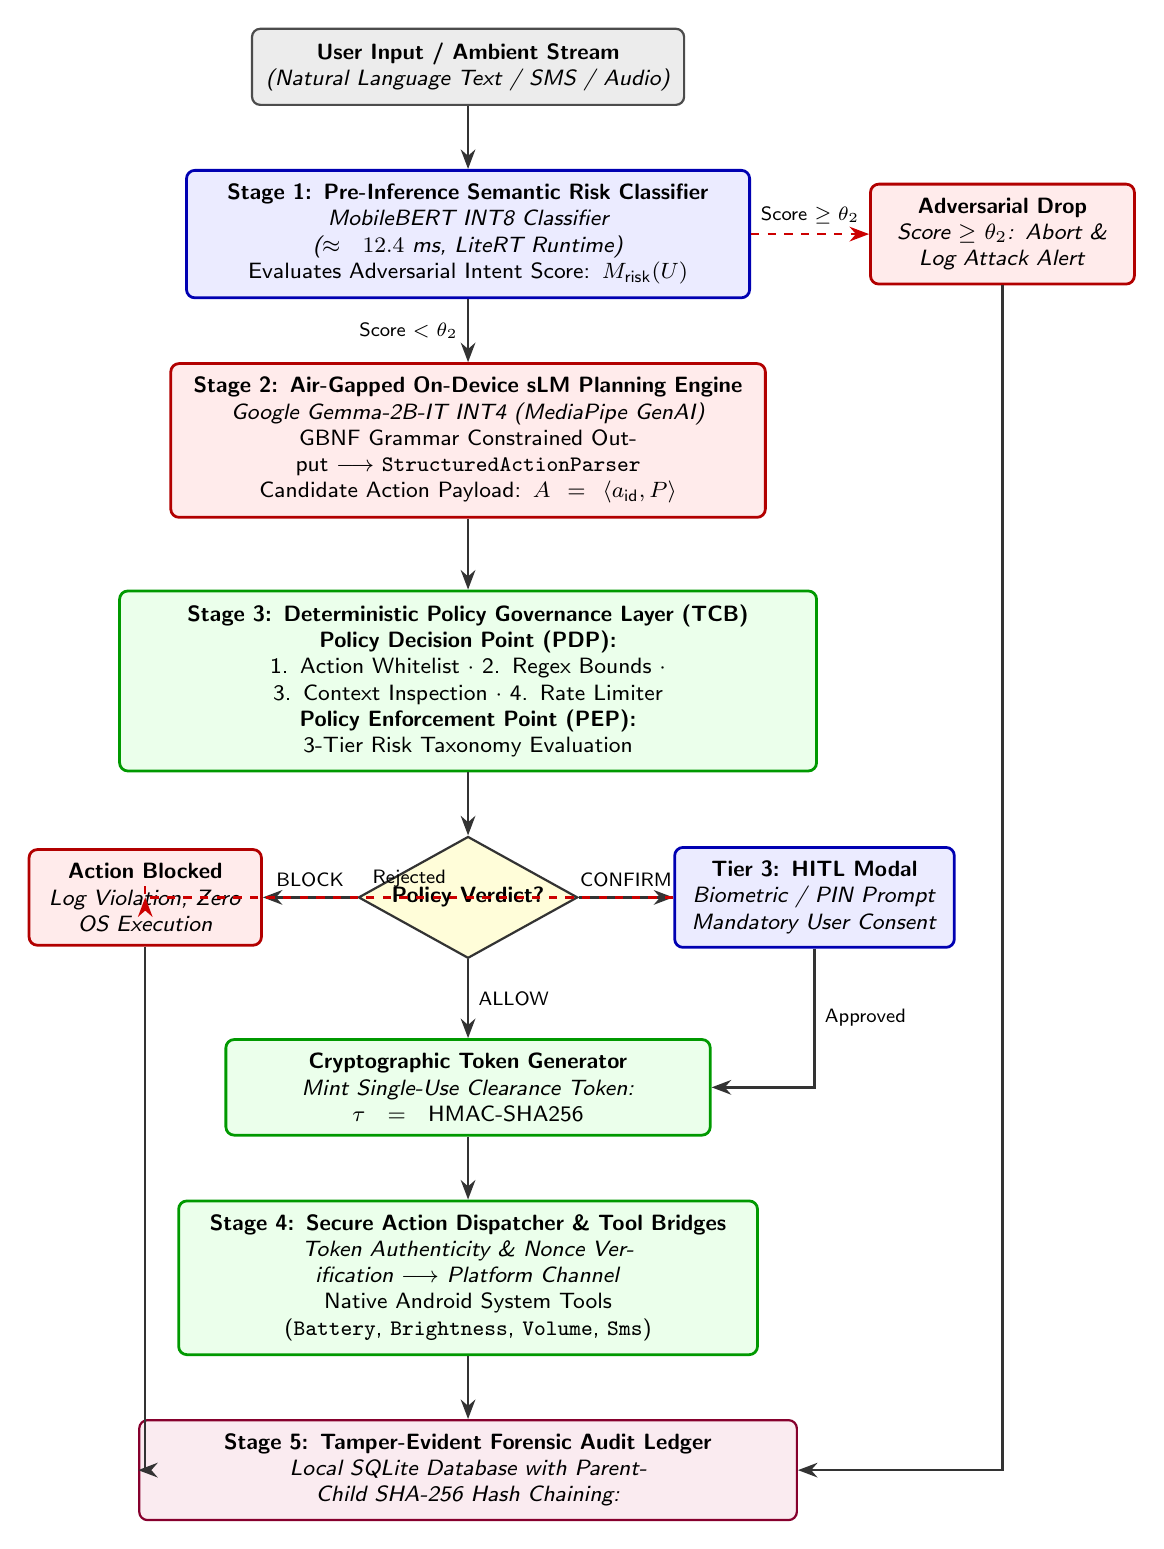
\begin{tikzpicture}[
    node distance=1.2cm and 1.0cm,
    every text node part/.style={align=center},
    font=\sffamily\footnotesize,
    % Styles
    box/.style={draw=black!70, fill=white, rounded corners=3pt, line width=0.8pt, inner sep=5pt, minimum height=0.9cm},
    untrusted/.style={box, fill=red!8, draw=red!70!black, line width=1pt},
    trusted/.style={box, fill=blue!8, draw=blue!70!black, line width=1pt},
    tcb/.style={box, fill=green!8, draw=green!60!black, line width=1pt},
    decision/.style={diamond, aspect=1.8, draw=black!80, fill=yellow!15, line width=0.8pt, inner sep=2pt},
    arrow/.style={-{Stealth[scale=1.0]}, line width=0.9pt, draw=black!80},
    dasharrow/.style={-{Stealth[scale=1.0]}, line width=0.9pt, dashed, draw=red!80!black}
]

% Inputs
\node (user) [box, fill=gray!15] {\textbf{User Input / Ambient Stream}\\\textit{(Natural Language Text / SMS / Audio)}};

% Stage 1: Pre-Inference Risk
\node (stage1) [trusted, below=0.8cm of user, text width=6.8cm] {\textbf{Stage 1: Pre-Inference Semantic Risk Classifier}\\\textit{MobileBERT INT8 Classifier ($\approx 12.4\text{ ms}$, LiteRT Runtime)}\\Evaluates Adversarial Intent Score: $M_{\text{risk}}(U)$};

% Drop Node
\node (drop) [untrusted, right=1.5cm of stage1, text width=3.0cm] {\textbf{Adversarial Drop}\\\textit{Score $\ge \theta_2$: Abort \&}\\\textit{Log Attack Alert}};

% Stage 2: AirGap sLM
\node (stage2) [untrusted, below=0.8cm of stage1, text width=7.2cm] {\textbf{Stage 2: Air-Gapped On-Device sLM Planning Engine}\\\textit{Google Gemma-2B-IT INT4 (MediaPipe GenAI)}\\GBNF Grammar Constrained Output $\longrightarrow$ \texttt{StructuredActionParser}\\Candidate Action Payload: $A = \langle a_{\text{id}}, P \rangle$};

% Stage 3: Policy Governance Layer
\node (pdp) [tcb, below=0.9cm of stage2, text width=8.5cm] {\textbf{Stage 3: Deterministic Policy Governance Layer (TCB)}\\
\textbf{Policy Decision Point (PDP):}\\
1. Action Whitelist $\cdot$ 2. Regex Bounds $\cdot$ 3. Context Inspection $\cdot$ 4. Rate Limiter\\
\textbf{Policy Enforcement Point (PEP):} 3-Tier Risk Taxonomy Evaluation};

% Fork Decision
\node (verdict) [decision, below=0.8cm of pdp] {\textbf{Policy Verdict?}};

% Left: Block
\node (block) [untrusted, left=1.2cm of verdict, text width=2.6cm] {\textbf{Action Blocked}\\\textit{Log Violation, Zero}\\\textit{OS Execution}};

% Right: HITL
\node (hitl) [trusted, right=1.2cm of verdict, text width=3.2cm] {\textbf{Tier 3: HITL Modal}\\\textit{Biometric / PIN Prompt}\\\textit{Mandatory User Consent}};

% Below: Token Mint
\node (mint) [tcb, below=1.0cm of verdict, text width=5.8cm] {\textbf{Cryptographic Token Generator}\\\textit{Mint Single-Use Clearance Token:}\\$\tau = \text{HMAC-SHA256}$};

% Stage 4: Dispatcher
\node (dispatcher) [tcb, below=0.8cm of mint, text width=7.0cm] {\textbf{Stage 4: Secure Action Dispatcher \& Tool Bridges}\\\textit{Token Authenticity \& Nonce Verification $\longrightarrow$ Platform Channel}\\Native Android System Tools (\texttt{Battery}, \texttt{Brightness}, \texttt{Volume}, \texttt{Sms})};

% Stage 5: Ledger
\node (ledger) [box, fill=purple!8, draw=purple!70!black, below=0.8cm of dispatcher, text width=8.0cm] {\textbf{Stage 5: Tamper-Evident Forensic Audit Ledger}\\\textit{Local SQLite Database with Parent-Child SHA-256 Hash Chaining:}};

% Connections
\draw [arrow] (user) -- (stage1);
\draw [arrow] (stage1) -- node[left] {\scriptsize Score $<\theta_2$} (stage2);
\draw [dasharrow] (stage1) -- node[above] {\scriptsize Score $\ge\theta_2$} (drop);
\draw [arrow] (stage2) -- (pdp);
\draw [arrow] (pdp) -- (verdict);
\draw [arrow] (verdict) -- node[above] {\scriptsize BLOCK} (block);
\draw [arrow] (verdict) -- node[above] {\scriptsize CONFIRM} (hitl);
\draw [arrow] (verdict) -- node[right] {\scriptsize ALLOW} (mint);
\draw [arrow] (hitl) |- node[right, near start] {\scriptsize Approved} (mint);
\draw [dasharrow] (hitl) -| node[above, near start] {\scriptsize Rejected} (block);
\draw [arrow] (mint) -- (dispatcher);
\draw [arrow] (dispatcher) -- (ledger);
\draw [arrow] (block) |- (ledger);
\draw [arrow] (drop) |- (ledger);

\end{tikzpicture}
\caption{Detailed Architectural Block Diagram.}
\label{fig:block_diagram}
\end{figure}

%------------------------------------------------------------------------------
\section{Module Description}
%------------------------------------------------------------------------------

The FLEK architecture comprises seven tightly integrated functional modules organized across the trust perimeter:

\subsection{Module 1: Pre-Inference Semantic Risk Classifier}
The semantic risk classifier operates at the outermost ingress boundary of the automation pipeline. Utilizing an 8-bit quantized MobileBERT architecture running inside Google LiteRT, this module analyzes the raw text query $U$ in $12.4 \pm 2.1\text{ ms}$ with a resident memory footprint of only $24.2\text{ MB}$. It computes an intent risk score mapping to one of three categories: Benign Utility ($0$), Sensitive / Privilege Request ($1$), or Adversarial Injection ($2$). Queries categorized as adversarial are terminated immediately before the system initializes autoregressive sLM decoding, thereby saving over $250\text{ ms}$ of generative compute and defending the mobile device against battery-depleting DoS loops.

\subsection{Module 2: Air-Gapped On-Device sLM Planning Engine}
Queries cleared by the risk classifier are passed to the on-device sLM engine. The host Android application operates in an air-gapped configuration, completely omitting the \texttt{android.permission.INTERNET} permission from its manifest. The engine runs a 4-bit quantized Google Gemma-2B-IT model using the Google MediaPipe GenAI SDK with GPU-accelerated OpenCL/Vulkan delegates. The model is prompted with a structured system prompt specifying registered tool schemas and constrained by a GBNF grammar forcing token emissions to adhere strictly to valid JSON key-value syntax.

\subsection{Module 3: Structured Action Parser and Syntax Healing State Machine}
Because quantized edge models occasionally experience generation cutoffs or token anomalies, the raw text output is processed by the \texttt{StructuredActionParser}. This module incorporates a 5-stage deterministic syntax healing state machine that:
\begin{enumerate}
    \item Strips Gemma-specific conversational turn tokens (\texttt{<start\_of\_turn>}, \texttt{<end\_of\_turn>}).
    \item Extracts JSON payloads from surrounding markdown code fences.
    \item Converts single-quoted strings and keys into standard double-quoted JSON formatting.
    \item Wraps unquoted dictionary keys and strips illegal trailing commas.
    \item Auto-closes truncated curly brackets and coerces string-encoded numerals into typed integers.
\end{enumerate}
If a payload cannot be repaired into a valid schema, it is automatically downgraded to `ActionType.unknown` and safely intercepted by the policy layer.

\subsection{Module 4: Deterministic Policy Governance Engine (PDP \& PEP)}
Implemented in Dart and Kotlin, this module serves as the primary security checkpoint between model planning and system execution:
\begin{itemize}
    \item \textbf{Policy Decision Point (PDP):} Evaluates four deterministic criteria:
    \begin{enumerate}
        \item \textit{Action Whitelist Verification:} Confirms that the requested action $a_{\text{id}}$ exists in the registered tool registry $\mathcal{A}_{\text{registered}}$. Unregistered tool calls trigger an immediate `BLOCK`.
        \item \textit{Parameter Boundary and Regex Validation:} Enforces type, range, and format constraints via dedicated validators (\texttt{NumericRangeValidator}, \texttt{EnumChoiceValidator}, \texttt{SecuritySanitizationValidator}). Numeric arguments (such as brightness and volume) must reside within $[0, 100]$, and phone numbers must match strict international E.164 regex patterns. Any payload containing \texttt{NaN}, \texttt{Infinity}, or shell injection tokens is blocked.
        \item \textit{Context-Aware State Inspection:} Interrogates live Android managers. If the device keyguard is locked ($s_{\text{lock}} = \text{LOCKED}$), actions attempting to launch apps or access private communications are rejected. Display brightness adjustments during night hours (22:00--06:00) are automatically capped.
        \item \textit{Sliding-Window Rate Limiter:} Implements a token-bucket rate limiter (maximum 10 requests per 60-second window) to neutralize automated looping attacks.
    \end{enumerate}
    \item \textbf{Policy Enforcement Point (PEP):} Manages a 3-tier risk taxonomy:
    \begin{itemize}
        \item \textit{Tier 1 (Low / Read-Only):} Auto-executed without user interruption (e.g., \texttt{GET\_BATTERY}, \texttt{GET\_TIME}).
        \item \textit{Tier 2 (Medium / Reversible):} Executed with an on-screen toast and audit ledger entry (e.g., \texttt{SET\_VOLUME}, \texttt{SET\_BRIGHTNESS}).
        \item \textit{Tier 3 (High / Destructive):} Execution is suspended until explicit user confirmation is obtained (e.g., \texttt{SEND\_SMS}, \texttt{DELETE\_FILE}).
    \end{itemize}
\end{itemize}

\subsection{Module 5: Human-in-the-Loop (HITL) Biometric Authorization Module}
When the PEP identifies a Tier 3 action, it invokes the Android Jetpack \texttt{BiometricPrompt} API. A secure, system-managed modal dialog appears on the screen, presenting the precise operational parameters (e.g., target phone number and SMS body). Execution resumes if and only if the genuine device owner authenticates successfully via biometric fingerprint or device PIN. User cancellation immediately drops the action and records a cancellation event in the audit store.

\subsection{Module 6: Secure Platform Channel Dispatcher and Native Tool Bridges}
Approved actions are transferred across Flutter Platform Channels (\texttt{MethodChannel} \texttt{"flek/native\_tools"}) to native Kotlin tool bridges. Crucially, the dispatcher validates the presence of an unconsumed, cryptographically authenticated clearance token $\tau$. Direct attempts by unauthorized code to invoke platform methods without a valid token result in immediate rejection. Upon validation, the bridge executes the corresponding Android API (\texttt{BatteryManager}, \texttt{AudioManager}, \texttt{Settings.System}, \texttt{SmsManager}, \texttt{AlarmClock}).

\subsection{Module 7: Tamper-Evident SHA-256 Forensic Audit Ledger}
Every pipeline transaction is logged into an on-device SQLite database. Each log entry incorporates the input query, risk score, sLM plan, policy evaluation metrics, cryptographic token hash, and execution outcome. Transactions are chained sequentially using SHA-256 hashing ($h_i = \text{SHA-256}(h_{i-1} \,\|\, r_i \,\|\, \tau_i)$), ensuring that any retroactive tampering with historical execution logs breaks the mathematical hash chain and triggers an alert in the application's Audit Studio.

%------------------------------------------------------------------------------
\section{Theoretical Foundation and Algorithms}
%------------------------------------------------------------------------------

\subsection{Mathematical Model and Threat Vectors}
The security posture of FLEK explicitly addresses six formal threat vectors $\mathcal{T} = \{\mathcal{T}_1, \mathcal{T}_2, \mathcal{T}_3, \mathcal{T}_4, \mathcal{T}_5, \mathcal{T}_6\}$:
\begin{itemize}
    \item $\mathcal{T}_1$ (\textit{Direct Prompt Injection}): Malicious user inputs designed to override system instructions.
    \item $\mathcal{T}_2$ (\textit{Indirect Prompt Injection}): Untrusted external data containing hidden agent commands.
    \item $\mathcal{T}_3$ (\textit{Unauthorized Privilege Escalation}): Hallucination of unregistered tools or ungranted OS permissions.
    \item $\mathcal{T}_4$ (\textit{Malicious Parameter Fuzzing}): Smuggling out-of-bounds, \texttt{NaN}, or script-injected parameter arguments.
    \item $\mathcal{T}_5$ (\textit{Context and State Invariant Violations}): Attempting sensitive operations under prohibited device states (e.g., locked keyguard).
    \item $\mathcal{T}_6$ (\textit{Denial-of-Service and Rapid Looping}): Automated execution bursts intended to drain battery or saturate carrier channels.
\end{itemize}

\subsection{Pre-Inference Risk Screening Formulation}
Let an incoming natural language prompt be denoted as $U \in \mathcal{U}$. The pre-inference classifier $M_{\text{risk}}: \mathcal{U} \to \{0, 1, 2\}$ evaluates $U$ against calibrated thresholds $\theta_1$ and $\theta_2$:
\begin{equation}
M_{\text{risk}}(U) = 
\begin{cases}
0 \text{ (Benign)}, & \text{if } \text{Score}(U) < \theta_1 \\
1 \text{ (Sensitive)}, & \text{if } \theta_1 \le \text{Score}(U) < \theta_2 \\
2 \text{ (Adversarial)}, & \text{if } \text{Score}(U) \ge \theta_2
\end{cases}
\end{equation}
If $M_{\text{risk}}(U) = 2$, the pipeline aborts immediately with an audit alert, bypassing sLM token generation.

\subsection{Structured Action and Context State Space}
For prompts where $M_{\text{risk}}(U) \in \{0, 1\}$, the sLM generates a candidate action:
\begin{equation}
A = \langle a_{\text{id}}, P \rangle, \quad P = \{ (k_1, v_1), (k_2, v_2), \dots, (k_m, v_m) \}
\end{equation}
where $a_{\text{id}} \in \mathcal{A}$ is the action identifier and $P$ represents parameter key-value pairs.

The dynamic mobile context at time $t$ is represented by the state tuple:
\begin{equation}
C = \langle s_{\text{lock}}, b_{\text{level}}, p_{\text{granted}}, t_{\text{tod}}, s_{\text{dnd}} \rangle
\end{equation}
where $s_{\text{lock}} \in \{\text{LOCKED}, \text{UNLOCKED}\}$ indicates screen keyguard status, $b_{\text{level}} \in [0, 100]$ denotes battery percentage, $p_{\text{granted}} \subseteq \mathcal{P}_{\text{OS}}$ represents currently granted Android permissions, $t_{\text{tod}}$ represents time of day, and $s_{\text{dnd}} \in \{\text{ACTIVE}, \text{INACTIVE}\}$ represents Do-Not-Disturb status.

\subsection{Deterministic Policy Decision Logic}
The Policy Decision Point implements evaluation function $\mathcal{D}(A, C) \to \{\text{ALLOW}, \text{CONFIRM}, \text{BLOCK}\}$:
\begin{equation}
\mathcal{D}(A, C) = 
\begin{cases}
\text{BLOCK}, & \text{if } \Phi_{\text{block}}(A, C) \\
\text{CONFIRM}, & \text{if } \Phi_{\text{confirm}}(A, C) \\
\text{ALLOW}, & \text{otherwise}
\end{cases}
\end{equation}
The blocking predicate $\Phi_{\text{block}}(A, C)$ evaluates to true if any structural, argument, contextual, or rate limit constraint is violated:
\begin{align}
\Phi_{\text{block}}(A, C) \iff & (a_{\text{id}} \notin \mathcal{A}_{\text{registered}}) \nonumber \\
& \lor \exists (k_i, v_i) \in P : \neg \text{Match}(v_i, \Pi(a_{\text{id}}, k_i)) \nonumber \\
& \lor (s_{\text{lock}} = \text{LOCKED} \land \neg \text{AllowLocked}(a_{\text{id}})) \nonumber \\
& \lor (\text{ReqPerm}(a_{\text{id}}) \nsubseteq p_{\text{granted}}) \nonumber \\
& \lor \text{RateLimitExceeded}(a_{\text{id}}, t)
\end{align}
where $\Pi(a_{\text{id}}, k_i)$ retrieves the strict regular expression constraint for parameter $k_i$. The confirmation predicate $\Phi_{\text{confirm}}(A, C)$ triggers HITL verification for Tier 3 actions or contextual escalations:
\begin{equation}
\Phi_{\text{confirm}}(A, C) \iff (\text{RiskTier}(a_{\text{id}}) = \text{TIER\_3}) \lor \text{Escalate}(A, C)
\end{equation}

\subsection{Cryptographic Token Clearance Protocol}
Upon approving an action, the policy engine issues a single-use cryptographic token:
\begin{equation}
\tau = \text{HMAC-SHA256}(K_{\text{device}}, a_{\text{id}} \,\|\, \text{Hash}(P) \,\|\, t_{\text{exp}} \,\|\, \text{nonce})
\end{equation}
where $K_{\text{device}}$ is an ephemeral key residing in the Android Hardware Keystore, $t_{\text{exp}}$ is an expiration timestamp ($<5$ seconds), and $\text{nonce}$ is a cryptographically random 128-bit integer. Tool execution occurs if and only if:
\begin{equation}
\text{VerifyToken}(\tau, A) = \text{TRUE} \quad \land \quad \text{IsUnconsumed}(\tau) = \text{TRUE}
\end{equation}

\subsection{Tamper-Evident Hash Chaining Invariant}
Every transaction is committed to the local audit ledger with SHA-256 parent-child hash linking:
\begin{equation}
h_i = \text{SHA-256}(h_{i-1} \,\|\, r_i \,\|\, \tau_i)
\end{equation}
where $r_i$ represents the full serialized transaction record, guaranteeing immutable non-repudiation.

\subsection{Formal Execution Algorithms}
The complete operational workflow is formalized in Algorithm~\ref{alg:secure_pipeline} and Algorithm~\ref{alg:pdp_evaluation}.

\begin{algorithm}[htbp]
\caption{End-to-End Secure Agent Execution Pipeline}
\label{alg:secure_pipeline}
\begin{algorithmic}[1]
\REQUIRE User prompt $U$, Device Context $C$, Audit Ledger $\mathcal{L}$
\ENSURE Execution Result $R$
\STATE $s \leftarrow M_{\text{risk}}(U)$ \COMMENT{Stage 1: Pre-inference screening}
\IF{$s = 2$}
    \STATE AppendAuditRecord($\mathcal{L}$, $U$, \text{null}, $\text{BLOCK}$, $\text{"ADVERSARIAL\_INPUT"}$)
    \RETURN $R \leftarrow \text{Error("Request aborted due to security risk.")}$
\ENDIF
\STATE $\hat{T} \leftarrow \text{MediaPipeGenerate}(\text{Gemma-2B-IT}, U)$ \COMMENT{Stage 2: sLM Planning}
\STATE $A \leftarrow \text{StructuredActionParser}(\hat{T})$ \COMMENT{Syntax healing \& schema extraction}
\IF{$A.a_{\text{id}} = \text{"UNKNOWN"}$}
    \RETURN $R \leftarrow \text{ConversationalFallback}(U)$
\ENDIF
\STATE $\text{verdict} \leftarrow \text{EvaluatePolicy}(A, C)$ \COMMENT{Stage 3: Policy evaluation (Algorithm 2)}
\IF{$\text{verdict} = \text{BLOCK}$}
    \STATE AppendAuditRecord($\mathcal{L}$, $U$, $A$, $\text{BLOCK}$, $\text{"POLICY\_VIOLATION"}$)
    \RETURN $R \leftarrow \text{Error("Action disallowed by policy governance.")}$
\ELSIF{$\text{verdict} = \text{CONFIRM}$}
    \STATE $\text{userApproved} \leftarrow \text{TriggerBiometricPrompt}(A)$
    \IF{$\neg \text{userApproved}$}
        \STATE AppendAuditRecord($\mathcal{L}$, $U$, $A$, $\text{BLOCK}$, $\text{"USER\_REJECTED"}$)
        \RETURN $R \leftarrow \text{Cancelled("Operation cancelled by user.")}$
    \ENDIF
\ENDIF
\STATE $\tau \leftarrow \text{MintClearanceToken}(A)$ \COMMENT{Mint cryptographic token}
\STATE $R \leftarrow \text{DispatchNativeAction}(A, \tau)$ \COMMENT{Stage 4: Token-verified native dispatch}
\STATE AppendAuditRecord($\mathcal{L}$, $U$, $A$, $\text{ALLOW}$, $R$) \COMMENT{Stage 5: Hash-chained audit}
\RETURN $R$
\end{algorithmic}
\end{algorithm}

\begin{algorithm}[htbp]
\caption{Deterministic Policy Decision Point (PDP) Evaluation}
\label{alg:pdp_evaluation}
\begin{algorithmic}[1]
\REQUIRE Candidate Action $A = \langle a_{\text{id}}, P \rangle$, Dynamic Context $C$
\ENSURE Policy Verdict $\in \{\text{ALLOW}, \text{CONFIRM}, \text{BLOCK}\}$
\IF{$a_{\text{id}} \notin \mathcal{A}_{\text{registered}}$}
    \RETURN $\text{BLOCK}$ \COMMENT{Unregistered action whitelist check}
\ENDIF
\FORALL{$(k_i, v_i) \in P$}
    \IF{$\neg \text{MatchRegex}(v_i, \Pi(a_{\text{id}}, k_i)) \lor \text{IsNaNOrInfinity}(v_i)$}
        \RETURN $\text{BLOCK}$ \COMMENT{Parameter boundary check}
    \ENDIF
\ENDFOR
\IF{$C.s_{\text{lock}} = \text{LOCKED} \land \neg \text{AllowLocked}(a_{\text{id}})$}
    \RETURN $\text{BLOCK}$ \COMMENT{Context keyguard invariant}
\ENDIF
\IF{$\text{ReqPerm}(a_{\text{id}}) \nsubseteq C.p_{\text{granted}}$}
    \RETURN $\text{BLOCK}$ \COMMENT{OS permission verification}
\ENDIF
\IF{$\text{CheckRateLimit}(a_{\text{id}}, \text{currentTime}) = \text{EXCEEDED}$}
    \RETURN $\text{BLOCK}$ \COMMENT{Sliding-window token bucket check}
\ENDIF
\IF{$\text{RiskTier}(a_{\text{id}}) = \text{TIER\_3} \lor \text{ContextEscalation}(A, C)$}
    \RETURN $\text{CONFIRM}$ \COMMENT{Mandatory Human-in-the-Loop tier}
\ENDIF
\RETURN $\text{ALLOW}$
\end{algorithmic}
\end{algorithm}


% Bibliography / References
\renewcommand\bibname{REFERENCES}
\clearpage
\phantomsection
\addcontentsline{toc}{chapter}{REFERENCES}
\nocite{*}
\printbibliography

\end{document}
